\section{Исходные данные}
\addcontentsline{toc}{section}{Исходные данные}	% Добавляем его в оглавление

\begin{table} [htbp]
  \centering
  \caption{Паспортные данные исследуемых транзисторов}
  \begin{tabular}{| c | c | c | c | c | c | c | c |}
    \hline
     \multirow{2}{*}{Транзистор} & \multirow{2}{*}{Тип} & \multirow{2}{*}{Корпус} & \multirow{2}{*}{$ h_{21_{\text{э}}} $ } & \multicolumn{4}{c|}{Предельные эксплуатационные параметры} \\ \cline{5-8}
    & & & & $ I_{\text{К}_{max}} $, мА & $ U_{\text{КЭ}_{max}} $, В & $ U_{\text{КБ}_{max}} $, В & $ P_{\text{К}_{max}}$, мВт \\
    \hline
    & & & & & & & \\
    \hline
  \end{tabular}

\end{table}

\begin{figure}[h]
  \center{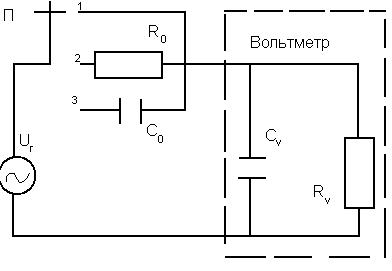
\includegraphics[width=0.8\linewidth]{scheme1}}
  \caption{Электрическая схема для исследования транзистора с общей базой}
\end{figure}

\clearpage
